\documentclass[10pt,a4paper]{article}
\usepackage[latin1]{inputenc}
\usepackage{amsmath}
\usepackage{amsfonts}
\usepackage{amssymb}
\usepackage{graphicx}

\begin{document}
\section{ASSIGNMENT NO: A3}
Author:\:   Ameeth Kanawaday\\
Roll No:\:  4430\\
\section{Problem Definition}
Lexical analyser for sample language using LEX.

\section{Learning Objectives:}
\begin{enumerate}
\item To understand concept of lexical analyser.
\item To use LEX as a lexical analyser generator.
\end{enumerate}

\section{S/W and H/W requirements:}
\begin{enumerate}
\item Open source 64 bit OS.
\item Gedit text editor.
\item flex.
\end{enumerate}

\section{Theory}
\textbf{Lexical Analysis:}
\\\\
Lexical analysis is the first phase of a compiler. It takes the modified source code from language preprocessors that are written in the form of sentences. The lexical analyzer breaks these syntaxes into a series of tokens, by removing any whitespace or comments in the source code.
\\If the lexical analyzer finds a token invalid, it generates an error. The lexical analyzer works closely with the syntax analyzer. It reads character streams from the source code, checks for legal tokens, and passes the data to the syntax analyzer when it demands.
\\\\
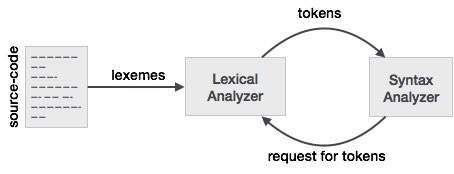
\includegraphics[scale=0.5]{im1.png}
\\\\
\textbf{Tokens:}
\\Lexemes are said to be a sequence of characters (alphanumeric) in a token. There are some predefined rules for every lexeme to be identified as a valid token. These rules are defined by grammar rules, by means of a pattern. A pattern explains what can be a token, and these patterns are defined by means of regular expressions.
\\In programming language, keywords, constants, identifiers, strings, numbers, operators and punctuations symbols can be considered as tokens.
\\\\
\textbf{Symbol Table:}
\\Symbol table is an important data structure created and maintained by compilers in order to store information about the occurrence of various entities such as variable names, function names, objects, classes, interfaces, etc. Symbol table is used by both the analysis and the synthesis parts of a compiler.
\\A symbol table may serve the following purposes depending upon the language in hand:
\begin{enumerate}
\item To store the names of all entities in a structured form at one place.
\item To verify if a variable has been declared.
\item To implement type checking, by verifying assignments and expressions in the source code are semantically correct.
\item To determine the scope of a name (scope resolution).
\end{enumerate}
A symbol table is simply a table which can be either linear or a hash table. It maintains an entry for each name in the following format.
\\<symbol name,  type,  attribute>
\\\\
\textbf{LEX:}
\\Lex is a program generator designed for lexical processing of character input streams. It accepts a high-level, problem oriented specification for character string matching, and produces a program in a general purpose language which recognizes regular expressions. The regular expressions are specified by the user in the source specifications given to Lex. The Lex written code recognizes these expressions in an input stream and partitions the input stream into strings matching the expressions. At the boundaries between strings program sections provided by the user are executed. The Lex source file associates the regular expressions and the program fragments. As each expression appears in the input to the program written by Lex, the corresponding fragment is executed. 
\\\\The user supplies the additional code beyond expression matching needed to complete his tasks, possibly including code written by other generators. The program that recognizes the expressions is generated in the general purpose programming language employed for the user's program fragments. Thus, a high level expression language is provided to write the string expressions to be matched while the user's freedom to write actions is unimpaired. This avoids forcing the user who wishes to use a string manipulation language for input analysis to write processing programs in the same and often inappropriate string handling language. 
\section{Related Mathematics}
Let S be the solution perspective of the given problem.
\\The set S is defined as:
\\$S=\lbrace\ s,e,X,Y,F,DD,NDD|\varnothing_{s}\rbrace$
\\Where,
\\s= Start point 
\\e= End point 
\\F= Set of main functions
\\DD= set of deterministic data
\\NDD= set of non deterministic data
\\\\X= Input Set.
\\X = $\lbrace source program code in high level language, matching rules \rbrace$
\\\\ Y = $\lbrace tokens, symbol table \rbrace$ 
\\\\ s = sample language ready into read buffer.
\\ e = tokens created and symbol table made.
\\\\ F = $\lbrace f_{read}, f_{match}, f_{st} \rbrace$
\\\\$f_{read}$  :function to read the sample language.
\\\\ $f_{match}$ :function to match the strings in sample language with the token rules.
\\\\ $f_{st}$ :function to add token information into symbol table.
\\\\ DD = $\lbrace sample code, matching rules \rbrace$
\\ NDD = $\phi$


\section{State Diagram}
\includegraphics[scale=0.5]{cl1a3.png}
\\q0 = read input code
\\q1 = token generation state
\\q2 = sysmbol table maintainance state
\\q3 = display symbol table state
\\qf = final state

\section{Program}
\begin{verbatim}

////main.c
#include<stdio.h>

int main() 
{
    int a = 1;
    printf("%d",a+5);
    return 0;
}


////main.l

%{
%}
%%
[ \t\n] {}
# {printf("#\t\tPreprocessor \n");}
include {printf("include\t\tkeyword\n");}
\< {printf("<\t\tleft angular bracket\n");}
\> {printf(">\t\tright angular bracket\n");}
[A-Za-z]+\.h {printf("%s\t\tC Library\n",yytext);}
int|short|float|long|double|char|string {printf("%s\t\tkeyword(datatype)\n",yytext);}
main { printf("main\t\tmain function\n"); } 
\( {printf("(\t\tleft circular bracket\n");}
\) {printf(")\t\tright circular bracket\n");}
\{ {printf("{\t\tleft curly bracket\n");}
\} {printf("}\t\tright curly bracket\n");}
printf {printf("printf\t\tprint function\n"); }
; {printf(";\t\tterminator\n");}
[A-Za-z]+[_A-Za-z0-9]* {printf("%s\t\tIdentifier\n",yytext); }
[0-9]+ {printf("%s\t\tInteger data\n",yytext);}
[0-9]+.[0-9]+ {printf("%s\t\tFloat data\n",yytext);}
\[ {printf("[\t\tLeft square bracket\n");}
\] {printf("]\t\tRight square bracket\n");}
[-+/*=&] {printf("%s\t\tOperator\n",yytext); }
\, {printf(",\t\tComma\n");}
\" {printf("\"\t\tQuotes\n");}
\"+[ A-Za-z0-9%]+\" {printf("%s\t\tMessage\n",yytext);}
%%
main()
{
yyin=fopen("main.c","r");
printf("-------------------------------------------------\n");
printf("Token\t\tDescription\n");
yylex();
printf("-------------------------------------------------\n");
}
int yywrap()
{
return 1;
}


OUTPUT:
ameeth@ubuntu-16.0.4:~/CL1$ lex main.l
ameeth@ubuntu-16.0.4:~/CL1$ gcc lex.yy.c -ll
ameeth@ubuntu-16.0.4:~/CL1$ ./a.out
-------------------------------------------------
Token		Description
#		Preprocessor 
include		keyword
<		left angular bracket
stdio.h		C Library
>		right angular bracket
int		keyword(datatype)
main		main function
(		left circular bracket
)		right circular bracket
{		left curly bracket
int		keyword(datatype)
a		Identifier
=		Operator
1		Integer data
;		terminator
printf		print function
(		left circular bracket
"%d"		Message
,		Comma
a		Identifier
+		Operator
5		Integer data
)		right circular bracket
;		terminator
return		Identifier
0		Integer data
;		terminator
}		right curly bracket
-------------------------------------------------
ameeth@ubuntu-16.0.4:~/CL1$ 


\end{verbatim}
\section{Conclusion}
Thus we successfully implemented LEX program for sample language and maintained a symbol table for it.
\end{document}